
\myChapter{Storia, Principi ed Operatori dei GA}
Nel seguente capitolo introdurremo gli algoritmi genetici mostrando brevemente la loro storia; per capire il principio su cui essi sono stati fondati e le loro caratteristiche peculiari ci baseremo su quanto scritto da Goldberg \cite{goldberg1} nella sua opera maggiormente conosciuta.
\section{Nascita e Principio}
Gli algoritmi genetici, pi\`u conosciuti nel mondo scientifico come GA, sono algoritmi di ricerca ed ottimizzazione introdotti per la prima volta da John Holland e dai suoi colleghi all'universit\`a del Michigan all'inizio degli anni '60, ed in seguito profondamente analizzati da David E. Goldberg nel suo libro "Genetic Algorithms in Search, Optimization \& Machine Learning" pubblicato nel 1989. Gli obiettivi principali della ricerca portata avanti da Holland e Goldberg sono stati in primo luogo astrarre e spiegare in modo rigoroso i processi adattativi dei sistemi naturali e, di conseguenza, costruire sistemi software in grado di conservare i meccanismi di tali sistemi.
\vspace{3mm}

I GA, com'\`e possibile dedurre dal loro nome, si basano sul principio darwiniano della sopravvivenza e riproduzione degli individui pi\`u idonei, attraverso lo scambio casuale, ma pur sempre strutturato, di informazioni volto alla creazione di algoritmi adattibili ad un'ampia  classe di problemi. Ad ogni generazione vengono creati nuovi individui a partire dai migliori di quelle precedenti ed i peggiori vengono rimpiazzati secondo logiche ben precise; al termine della riproduzione vengono valutati i vari individui, ai quali viene assegnato un valore di idoneit\`a, necessario per lo sviluppo delle successive generazioni.

La grande sfida che la ricerca sugli algoritmi genetici si pone \`e la \textit{robustezza}, ovvero l'equilibrio fra efficienza ed efficacia necessario per la riuscita, sopravvivenza e miglioramento nei vari ambiti di applicazione dei GA; la robustezza implica una diminuzione, o la totale eliminazione, dei costi di re-design di un sistema e maggiore \`e essa pi\`u a lungo ed in modo migliore i sistemi potranno comportarsi. \`E meraviglioso accorgersi di come il parametro della robustezza sia presente ovunque nei sistemi naturali, nei quali vigono regole di auto-miglioramento, auto-riparazione e riproduzione attraverso le meccaniche della selezione naturale; questo meccanismo \`e praticamente sconosciuto nel mondo dei sistemi artificali, ma \`e prorio qui che entrano in scena i GA.
\section{Caratteristiche Peculiari}
Secondo quanto stabilito da Goldberg in \cite{goldberg1}, nella ricerca della robustezza i GA differiscono molto dalle pi\`u note procedure di ricerca ed ottimizzazione particolarmente per quattro motivi:
\begin{enumerate}
    \item I GA lavorano tramite codifiche di un insieme di parametri, non con i parametri stessi.
    \item I GA cominciano la loro ricerca da una popolazione di punti, non da uno solo.
    \item I GA usano una funzione oggettiva per la valutazione delle informazioni ottenute, non hanno bisogno di dati ausiliari.
    \item I GA usano regole dettate dalla probabilit\`a, non sono deterministici.
\end{enumerate}
Come si pu\`o osservare dal primo punto elencato, gli algoritmi genetici hanno bisogno che l'insieme di parametri di un problema di ricerca e/o ottimizzazione sia codificato come un insieme di stringhe definite su un alfabeto finito.

Consideriamo, come fatto da Goldberg stesso nella sua opera \cite{goldberg1}, una scatola chiusa con sette interruttori che agiscono da input, per ogni combinazione esiste un segnale di output f che in termini matematici pu\`o essere espresso come f(i), dove i \`e una qualunque combinazione dei sette interrutori; l'obiettivo del problema consiste nell'impostare gli interruttori in modo da ottenere il massimo valore che f pu\`o assumere; con i GA per prima cosa codifichiamo gli interruttori stessi come una stringa: la soluzione pi\`u semplice prevede di implementare una stringa di sette valori binari dove l'1 rappresenta il segnale ON e lo 0 il segnale OFF: per esempio la stringa 1001110, rappresenta la combinazione in cui il secondo, il terzo e l'ultimo interruttore sono spenti.
\begin{figure}[H]
    \centering
    \hfill
    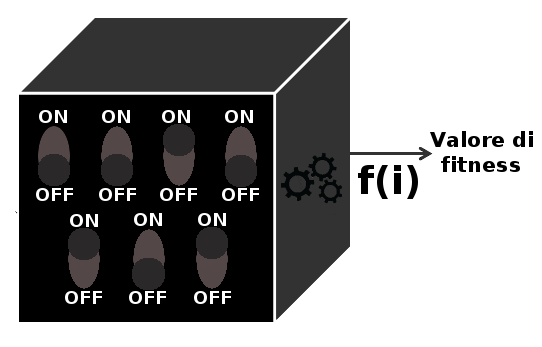
\includegraphics[width=0.85\textwidth]{Images/immagine1.png}
    \hspace*{\fill}
    \caption{I GA hanno bisogno solamente di una codifica e di una funzione di fitness per il loro funzionamento, a loro non interessano i meccanismi interni al problema.}
    \label{fig:box_switches}
\end{figure}
Come suggerito dal punto 2, gli algoritmi genetici cominciano con una popolazione di invidividui (in questo caso, stringhe) e da esse vengono prodotte le generazioni successive, nel problema preso in considerazione una combinazione casuale di partenza potrebbe essere data dal lancio di una moneta (testa == $1$, croce == $0$) con dimensione delle popolazione uguale a 5 (cifra molto esigua per gli standard dei GA):\vspace{3mm}
\break
$1010110\break
0001101\break
1100010\break
1110101\break
0010001$\vspace{3mm}

Dopo di ci\`o, le successive popolazioni sono generate attraverso i vari passi dell'algoritmo genetico (andremo nel dettaglio nella prossima sezione), il quale non richiede altre informazioni per operare, di fatto si potrebbe dire che i GA sono \textit{ciechi}: per raggiungere il loro obiettivo hanno solo bisogno di un valore di payoff associato ad ognuna delle stringhe della popolazione, nel caso da noi preso in esame altro non \`e che la funzione f(i). Questo rende l'approccio coi GA molto pi\`u semplice rispetto ai suoi concorrenti, ma, d'altro canto, il rifiuto di usare conoscenze specifiche laddove possibile potrebbe limitare le performance di un GA nel caso si trovasse faccia a faccia con metodi specifici per un dato problema.
\vspace{3mm}

Il punto 4, per concludere, sottolinea che i GA usano regole probabilistiche per guidare la propria ricerca, questo potrebbe far storcere il naso a molti, dato che siamo abituati a lavorare per la maggior parte del nostro tempo con metodi deterministici; l'uso della probabilit\`a non implica che i GA siano un semplice metodo di ricerca fondato sulla pura casualit\`a: la presa di una decisione non avviene tramite il semplice lancio di una moneta, la ricerca \`e di fatto guidata verso la soluzione migliore; \textit{la probabilit\'a svolge soltanto un ruolo di strumento necessario per l'attuazione}.

Prese in considerazione le quattro differenze elencate all'inizio di questa sezione, entreremo maggiormente in dettaglio nell'esecuzione di un algoritimo genetico nella prossima sezione attraverso la dettagliata descrizione delle sue funzioni principali.
\section{Glossario ed Operatori Fondamentali}
I meccanismi di un GA sono estremamente semplici, in quanto si basano nientemeno che sulla copia di stringhe e sullo scambio di sottostringhe, ma la ragione per cui questo processo non risulta arduo \`e ancora pi\`u sottile e potente; la facilit\`a delle operazioni da eseguire sulle stringhe e la loro efficacia sono i maggiori punti di forza dei GA.
\vspace{3mm}

Prima di addentrarci nella descrizione dei meccanismi di un GA occorre introdurre i termini \cite{goldberg1}, derivanti in gran parte dalla biologia, che ci accompagneranno per tutta la tesi:
\begin{enumerate}
    \item \textbf{Cromosoma}; codifica di una delle soluzioni al problema preso in esame, rappresentato come una stringa numerica/alfanumerica a seconda del contesto. La lunghezza delle stringa \`e strettamente correlata al problema (si noti l'esempio portato nella sezione 2.2).
    \item \textbf{Popolazione}; insieme di individui, quest'ultimi rappresentati da cromosomi e, dunque, altro non \`e che il set complessivo delle soluzioni ad un problema.
    \item \textbf{Gene}; parte di un cromosoma, corrispondente ad un elemento della stringa.
    \item \textbf{Allele}; il valore che un gene pu\`o assumere, nel caso di stringhe binarie gli alleli sono $0$ ed $1$.
    \item \textbf{Locus}; posizione di un gene nella stringa, nella maggioranza dei casi useremo questo termine con lo stesso significato di gene.
    \item \textbf{Fitness o Idoneit\`a}; grado di idoneit\`a di una particolare soluzione al problema dato. Tale valore \`e generato da un'apposita \textit{funzione di fitness} ad hoc.
\end{enumerate}
Armati di questi termini possiamo, a questo punto, vedere nel dettaglio gli operatori (le cui innumerevoli varianti sono state approfonditamente illustrate in \cite{glossary}) che definiscono i GA come tali.
\subsection{Selezione}
Operatore conosciuto anche come \textit{riproduzione}, \`e un processo nel quale le stringhe di una data popolazione sono copiate rispetto al valore obiettivo di una funzione di fitness f, la quale pu\`o essere vista (nei casi noti della vita di tutti i giorni) come una misura di un profitto od utilit\`a che desideriamo massimizzare.
Copiare le stringhe a seconda del loro valore di fitness comporta una maggiore probabilit\`a, per quelle stringhe che hanno ottenuto i pi\`u alti risultati, di contribuire alla generazione della prossima popolazione.

La selezione altro non \`e che la versione artificiale del pi\`u famoso meccanismo darwiniano della selezione naturale: in quest'ultimo caso il fitness di una popolazione proviene dalle capacit\`a di sopravvivenza di una specie, mentre nel nostro sistema artificiale \`e dato da una funzione oggettiva che determina la vita o la morte di una stringa.
\vspace{3mm}

L'operatore di selezione pu\`o essere implementato in forma algoritmica in base a numerose tecniche \cite{glossary} \cite{selection2}, di seguito sono presentate quelle pi\`u conosciute:
\begin{itemize}
    \item \textbf{Casuale:} forma pi\`u semplice in assoluto, ma meno efficiente; data una popolazione di dimensione N, una stringa ha probabilit\`a di riproduzione pari a \(\frac{1}{N}\).
    \item \textbf{A roulette:} sia N la dimensione della popolazione e \(f\ped{i}\) il valore di fitness dell'i-esima stringa, allora la probabilit\`a con la quale essa potrebbe essere scelta corrisponde a: $$p\ped{i}=\frac{f\ped{i}}{\sum_{j=1}^{N} f\ped{j}}$$
    \item \textbf{Rapportato al migliore:} siano N ed f\ped{i} definiti come in precedenza e sia f\ped{M} il valore massimo di fitness ottenuto ad una determinata generazione, un individuo pu\`o essere selezionato con probabilit\`a: $$p\ped{i}=\frac{f\ped{i}}{f\ped{M}}$$In questo caso l'individuo migliore sar\`a sempre in grado di partecipare al crossover.
    \item \textbf{A categoria:} simile alla prima, ma vengono considerate tutte le coppie possibili di individui, computazionalmente non efficiente dato che potrebbe trovarsi in stallo nel caso in cui ci fossero due coppie con valori di fitness molto vicine fra loro.
    \item \textbf{A torneo \cite{selection1}:} prevede lo svolgimento di "tornei" fra pochi cromosomi scelti in modo casuale dalla popolazione; il vincitore di ciascun "torneo" \`e scelto per il crossover, pi\`u la dimensione del torneo \`e maggiore meno probabile sar\`a la scelta di un individuo con fitness bassa, dato che aumentano le possibilit\`a che un cromosoma con alta fitness partecipi al torneo.
    
    L'algoritmo funziona pressapoco nel seguente modo:
    \begin{enumerate}
        \item seleziona k (dimensione del torneo) individui dalla popolazione in modo casuale;
        \item scelta del miglior cromosoma dal torneo con probabilit\`a p;
        \item scelta del secondo miglior cromosoma con probabilit\`a $$p*(1-p)$$
        \item scelta del terzo miglior cromosoma con  probabilit\`a $$p*(1-p)^2$$
        \item scelta dell'iesimo miglior cromosoma con probabilit\`a $$p*(1-p)^{(i-1)}$$ e cos\`i via fino a raggiungere il k-esimo elemento;
    \end{enumerate}
    Rispetto alle precedenti forme, la selezione a torneo risulta pi\`u semplice e lavora efficaciemente su architetture parallele, oltre ad essere indipendente da funzioni di fitness scalari; si noti che con k=1 si ottiene una selezione casuale.
\end{itemize}
\subsection{Crossover}
L'operatore di crossover si occupa dello scambio di informazioni fra due individui della popolazione che hanno superato la fase di selezione con l'obiettivo di produrre prole, la quale potrebbe avvicinarsi alla soluzione richiesta. 
Prendiamo come esempio il crossover semplice (scelta casuale di due individui che hanno superato la selezione attraverso l'apposito operatore) e mostriamo come esegue il proprio compito.%il quale non \`e detto che avvenga ad ogni iterazione del GA (esiste una frequenza di crossover p\ped{c}), e mostriamo come esso esegue il proprio lavoro.
\vspace{3mm}

Se l \`e la dimensione dei cromosomi, sia k intero scelto in modo casuale nell'intervallo [1, l-1] e rappresentante il \textit{punto di crossover} da cui due individui si scambieranno i propri geni; lo scambio avviene, nella variante pi\`u semplice, fra le posizioni [k+1, l] e da esso saranno generati due nuovi cromosomi. Per avere un'idea migliore del funzionamento, mostriamo i vari tipi di crossover con annessa figura esplicativa:
\begin{itemize}
    \item\textbf{Casuale:} per ciascuna coppia di geni viene generato un numero intero fra $0$ ed $1$, se il numero risulta $1$ allora il cromosoma figlio erediter\`a il gene del primo individuo, altrimenti riceve il gene dal secondo. Questa forma di crossover distribuisce in modo casuale i geni dei genitori, risulta la meno efficiente fra quelle esposte.
    \begin{figure}[H]
        \centering
        \hfill
        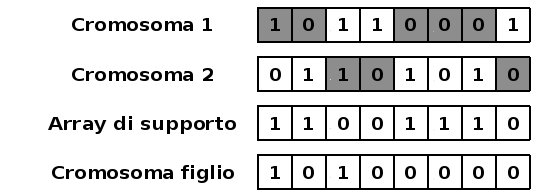
\includegraphics[width=0.95\textwidth]{Images/CrossoverRandom.png}
        \hspace*{\fill}
        %\caption{I GA hanno bisogno solamente di una codifica e di una funzione di fitness per il loro funzionamento, a loro non interessano i meccanismi interni al problema.}
        \caption{Crossover casuale}
        \label{fig:randomcrossover}
    \end{figure}
    \item \textbf{A punto singolo:} variante spiegata nel breve esempio introduttivo, gli array rappresentanti i cromosomi vengono "tagliati" ad un punto di crossover k, determinato in modo casuale o predefinito; il primo figlio sar\`a dato dalla combinazione dei primi k geni del primo individuo e dai restanti l-k geni del secondo, il secondo figlio sar\`a generato in modo quasi simmetrico (testa del secondo cromosoma e coda del primo).
    \begin{figure}[H]
        \centering
        \hfill
        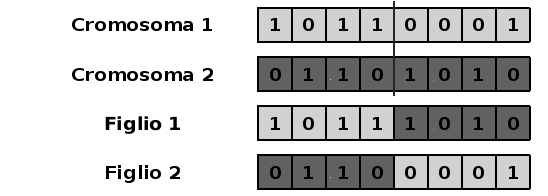
\includegraphics[width=0.95\textwidth]{Images/CrossoverSinglePoint.png}
        \hspace*{\fill}
        %\caption{I GA hanno bisogno solamente di una codifica e di una funzione di fitness per il loro funzionamento, a loro non interessano i meccanismi interni al problema.}
        \caption{Crossover a punto singolo}
        \label{fig:singlepointcrossover}
    \end{figure}
    \item \textbf{A punto doppio:} variante del precedente, vi sono, come dice il nome, due punti di crossover k e j, la figura 4 mostra molto semplicemente il suo funzionamento.
    \begin{figure}[H]
        \centering
        \hfill
        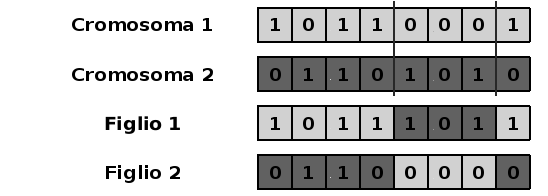
\includegraphics[width=0.95\textwidth]{Images/CrossoverDoublePoints.png}
        \hspace*{\fill}
        %\caption{I GA hanno bisogno solamente di una codifica e di una funzione di fitness per il loro funzionamento, a loro non interessano i meccanismi interni al problema.}
        \caption{Crossover a punto doppio}
        \label{fig:doublepointcrossover}
    \end{figure}
\end{itemize}
Per terminare la sezione, vorremmo far notare che il crossover fra due cromosomi, a differenza della selezione, non avviene ad ogni iterazione del GA, ma ha una frequenza pari a p\ped{c}, arbitrariamente scelta dal programmatore. 
\subsection{Mutazione}
L'ultimo operatore che caratterizza i GA consiste nella mutazione: nei sistemi naturali essa viene definita come un'anomalia nel corredo genetico di un individuo che potrebbe causare miglioramenti o peggioramenti nelle condizioni di vita, nei sistemi artificiali (nel nostro specifico interesse, nei GA) consiste nella modifica dei geni di cromosoma in base ad un coefficiente di mutazione p\ped{m} definito all'inizio del programma.
%\vspace{3mm}

La mutazione ha il compito di migliorare il valore di fitness di un individuo e/o ampliare lo spazio di ricerca nel problema, in modo da non cadere e rimanere in ottimi locali, punto di debolezza dei GA, di cui parlaremo in un apposito capitolo.

Passata una stringa all'operatore, quest'ultimo pu\`o cambiare ogni singolo gene con coefficiente p\ped{m}; \`e evidente il fatto che un valore troppo alto di p\ped{m} possa portare su una strada sbagliata il GA, mentre un valore estremamente basso non influisce in alcun modo sull'andamento dell'algoritmo.
\newpage